\documentclass[12pt]{article}
\usepackage[margin=1in]{geometry}
\usepackage{tikz}
\usepackage{xcolor}
\usepackage{amssymb}
\usetikzlibrary{shapes.geometric, arrows, positioning, fit, backgrounds}

\begin{document}

\begin{figure}[h]
\centering
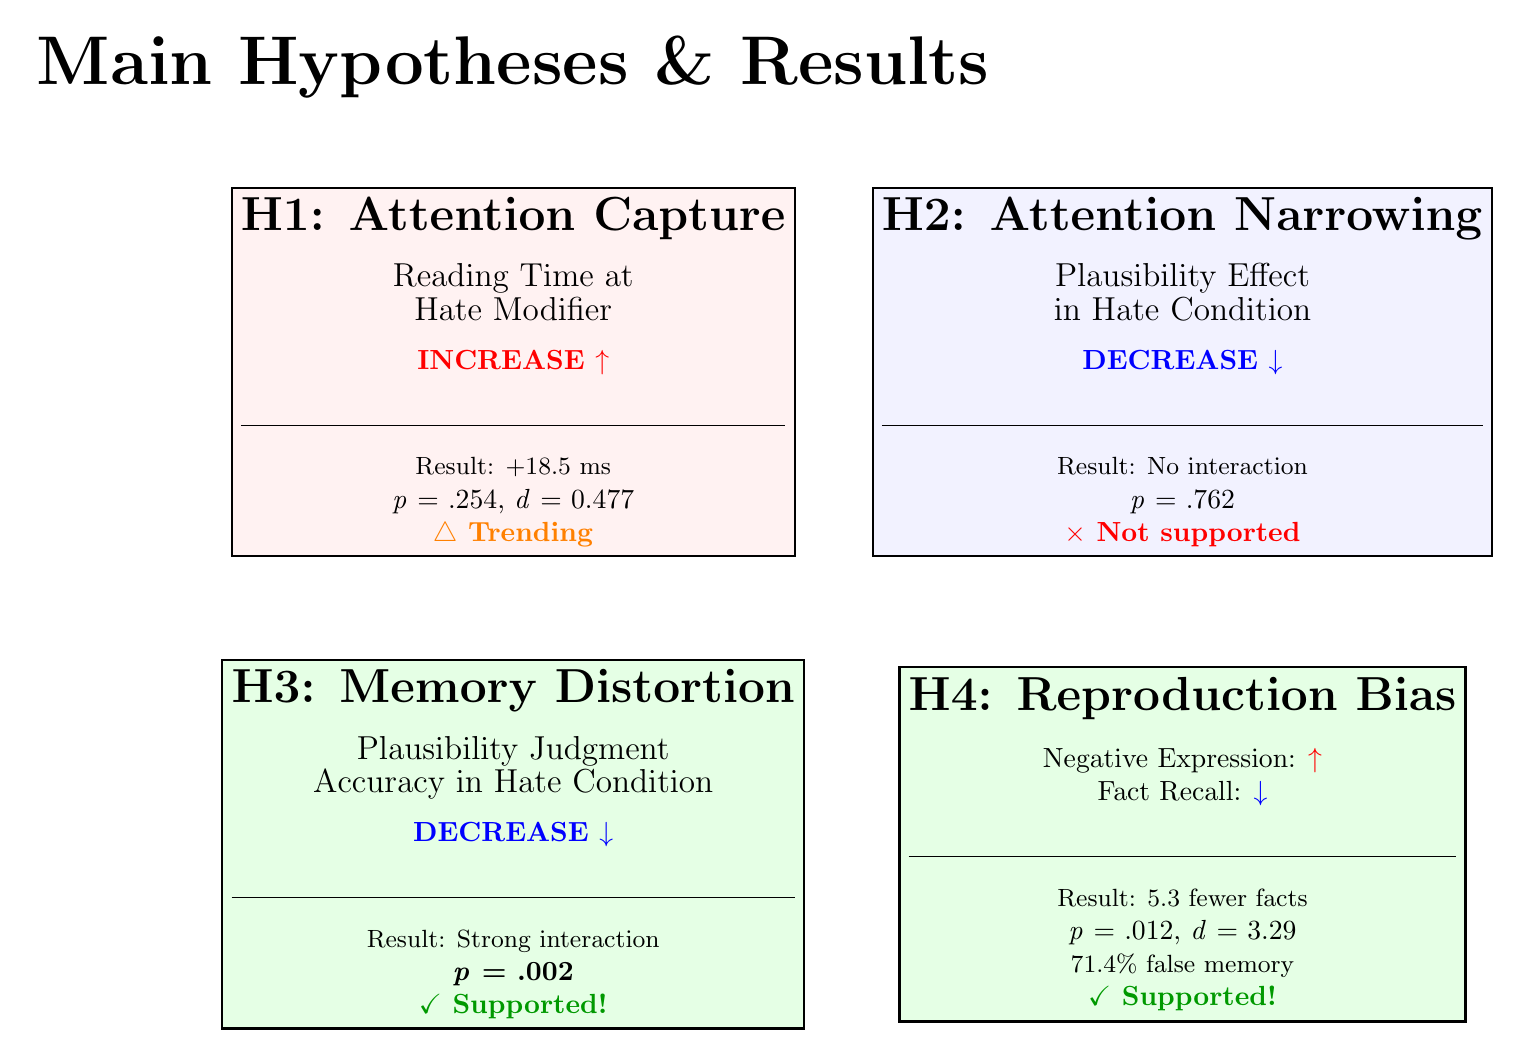
\begin{tikzpicture}[
    node distance=0.5cm,
    box/.style={rectangle, draw, minimum width=7cm, minimum height=4.5cm, thick, align=center},
    title/.style={font=\Large\bfseries},
    hypothesis/.style={font=\large},
    arrow/.style={->, >=stealth, line width=1.5mm},
    up/.style={arrow, red},
    down/.style={arrow, blue},
    result/.style={font=\normalsize\bfseries}
]

% H1: Top-left
\node[box, fill=red!5] (h1) at (0,6) {
    \textbf{\LARGE H1: Attention Capture}\\[0.3cm]
    \large Reading Time at\\
    \large Hate Modifier\\[0.2cm]
    \normalsize \textcolor{red}{\textbf{INCREASE $\uparrow$}}\\[0.3cm]
    \hrulefill\\[0.2cm]
    \small Result: +18.5 ms\\
    \textit{p} = .254, \textit{d} = 0.477\\
    \textcolor{orange}{\textbf{$\triangle$ Trending}}
};

% H2: Top-right
\node[box, fill=blue!5] (h2) at (8.5,6) {
    \textbf{\LARGE H2: Attention Narrowing}\\[0.3cm]
    \large Plausibility Effect\\
    \large in Hate Condition\\[0.2cm]
    \normalsize \textcolor{blue}{\textbf{DECREASE $\downarrow$}}\\[0.3cm]
    \hrulefill\\[0.2cm]
    \small Result: No interaction\\
    \textit{p} = .762\\
    \textcolor{red}{\textbf{$\times$ Not supported}}
};

% H3: Bottom-left
\node[box, fill=green!10] (h3) at (0,0) {
    \textbf{\LARGE H3: Memory Distortion}\\[0.3cm]
    \large Plausibility Judgment\\
    \large Accuracy in Hate Condition\\[0.2cm]
    \normalsize \textcolor{blue}{\textbf{DECREASE $\downarrow$}}\\[0.3cm]
    \hrulefill\\[0.2cm]
    \small Result: Strong interaction\\
    \textbf{\textit{p} = .002}\\
    \textcolor{green!60!black}{\textbf{$\checkmark$ Supported!}}
};

% H4: Bottom-right
\node[box, fill=green!10] (h4) at (8.5,0) {
    \textbf{\LARGE H4: Reproduction Bias}\\[0.3cm]
    \normalsize Negative Expression: \textcolor{red}{\textbf{$\uparrow$}}\\
    \normalsize Fact Recall: \textcolor{blue}{\textbf{$\downarrow$}}\\[0.3cm]
    \hrulefill\\[0.2cm]
    \small Result: 5.3 fewer facts\\
    \textit{p} = .012, \textit{d} = 3.29\\
    \small 71.4\% false memory\\
    \textcolor{green!60!black}{\textbf{$\checkmark$ Supported!}}
};

% Add large arrows
\begin{scope}[on background layer]
    % H1 up arrow
    \draw[up] (-2.8,7.8) -- (-2.8,6.2);

    % H2 down arrow
    \draw[down] (5.7,7.8) -- (5.7,6.2);

    % H3 down arrow
    \draw[down] (-2.8,1.8) -- (-2.8,0.2);

    % H4 double arrows (up and down)
    \draw[up] (5.9,1.8) -- (5.9,0.8);
    \draw[down] (5.9,0.5) -- (5.9,-0.5);
\end{scope}

% Add section title
\node[above=1cm of h1.north, anchor=south, font=\Huge\bfseries] {Main Hypotheses \& Results};

\end{tikzpicture}
\caption{Overview of four main hypotheses with predicted effects and empirical results. Red arrows ($\uparrow$) indicate predicted increases; blue arrows ($\downarrow$) indicate predicted decreases.}
\end{figure}

\newpage

\section*{Detailed Hypothesis Descriptions}

\subsection*{H1: Attention Capture}

\textbf{Prediction:} Hate modifiers will elicit \textcolor{red}{longer reading times ($\uparrow$)} than neutral modifiers, reflecting affect-driven attentional capture.

\textbf{Result:}
\begin{itemize}
    \item Original data: +7.2 ms, \textit{p} = .468, \textit{d} = 0.293
    \item With outlier removal (200--1600ms): +18.5 ms, \textit{p} = .254, \textit{d} = 0.477
\end{itemize}

\textbf{Status:} Trending effect in predicted direction (effect size increases 63\% with stricter outlier criteria)

\textbf{Interpretation:} Direction consistent with hypothesis. Single outlier (1725 ms) substantially influenced results, demonstrating importance of data quality control.

\subsection*{H2: Attention Narrowing \& Shallow Integration}

\textbf{Prediction:}
\begin{itemize}
    \item Neutral-modifier sentences: Clear plausibility effect (Implausible > Plausible RT)
    \item Hate-modifier sentences: \textcolor{blue}{Reduced plausibility effect ($\downarrow$)}, indicating shallower semantic integration under attentional narrowing
\end{itemize}

\textbf{Result:}
\begin{itemize}
    \item Neutral context: NI -- NP = +7.06 ms
    \item Hate context: HI -- HP = +7.10 ms
    \item Interaction: \textit{F}(1,6) = 0.00, \textit{p} = .995
\end{itemize}

\textbf{Status:} Not supported

\textbf{Interpretation:} No evidence of attention narrowing effect. Possible reasons: (1) small sample size (N=7), (2) weak plausibility manipulation, (3) need to examine spillover region.

\subsection*{H3: Biased Memory (Trade-off + Distortion)}

\textbf{Prediction:} Relative to neutral context, hate context will lead to \textcolor{blue}{lower accuracy ($\downarrow$)} for plausibility discrimination in recognition memory.

\textbf{Result:}
\begin{itemize}
    \item \textbf{Strong Emotion $\times$ Plausibility interaction: \textit{p} = .002}
    \item Neutral condition: Clear discrimination (P -- I = +0.593, \textit{p} = .001) $\checkmark$
    \item Hate condition: No discrimination (P -- I = --0.171, \textit{p} = .439) $\times$
\end{itemize}

\textbf{Status:} \textcolor{green!60!black}{\textbf{Strongly supported!}}

\textbf{Interpretation:} Hate speech disrupts accurate encoding and retrieval of plausibility information. Exact replication of previous dataset (\textit{p} = .002 in both datasets). Distortion index shows 5/7 participants exhibited expected pattern.

\subsection*{H4: Encoding Bias in Reproduction}

\textbf{Prediction:} Free descriptions after hate context will contain:
\begin{itemize}
    \item \textcolor{red}{Higher proportion ($\uparrow$)} of hate-consistent propositions and negative adjectives
    \item \textcolor{blue}{Fewer neutral background details ($\downarrow$)}
\end{itemize}

\textbf{Result:}
\begin{itemize}
    \item \textbf{Negative expression users recalled 5.3 fewer facts} (2.5 vs.\ 7.8 facts)
    \item Independent samples \textit{t}-test: \textit{t}(5) = 3.22, \textbf{\textit{p} = .012}, Cohen's \textit{d} = 3.29
    \item \textbf{71.4\% of participants included false information} (implausible content recalled as fact)
    \item Mean false information: 2.29 instances per participant
\end{itemize}

\textbf{Status:} \textcolor{green!60!black}{\textbf{Supported!}}

\textbf{Critical Methodological Finding:}
\begin{itemize}
    \item All negative expressions (100\%) were \textit{indirect}: ``unsophisticated'' ({\fontfamily{lmr}\selectfont\emph{cheonbak}}), ``ignorant'' ({\fontfamily{lmr}\selectfont\emph{muji}}), ``low-level'' ({\fontfamily{lmr}\selectfont\emph{sujun nat}})
    \item Zero direct hate speech reproduced
    \item Suggests hate speech induces \textbf{schema-level implicit bias} rather than explicit word copying
    \item Social desirability prevents direct hate reproduction, but fundamental negative attitude persists through indirect language
\end{itemize}

\section*{Summary Table}

\begin{table}[h]
\centering
\begin{tabular}{|l|l|c|c|c|}
\hline
\textbf{Hypothesis} & \textbf{Measure} & \textbf{Result} & \textbf{\textit{p}-value} & \textbf{Status} \\ \hline
Manipulation & Negativity rating & \textit{d} = 4.18 & < .0001 & \checkmark \checkmark \checkmark \\ \hline
H1 (original) & Modifier RT & +7.2 ms & .468 & $\triangle$ \\ \hline
H1 (strict) & Modifier RT & +18.5 ms & .254 & $\triangle$ \\ \hline
H2 & Interaction & +7.1 ms & .762 & $\times$ \\ \hline
H3 & Interaction & +0.734 & \textbf{.002} & \checkmark \checkmark \\ \hline
H4 & Fact recall diff & --5.3 facts & \textbf{.012} & \checkmark \checkmark \\ \hline
H4 & False memory & 71.4\% & --- & \checkmark \\ \hline
\end{tabular}
\caption{Summary of hypothesis testing results. $\checkmark$ = supported, $\triangle$ = trending, $\times$ = not supported}
\end{table}

\end{document}
